\documentclass{article}

\usepackage{amsmath}
\usepackage{minted}
\usepackage[ruled,vlined]{algorithm2e}
\usepackage[utf8]{inputenc}
\usepackage[english]{babel}
\usepackage{blindtext}
\usepackage{amssymb}
\usepackage{scrextend}
\usepackage{multicol}
\usepackage{wrapfig}
\usepackage{tikz}

\usepackage{amsthm}

\usepackage[margin=1in]{geometry}

\title{\vspace{-3cm}Homework 4}
\author{Yutong Huang (yxh589)}
\date{}

\begin{document}
\maketitle

\section*{Problem 1}
\subsection*{(a)}
\begin{center}
    \begin{tikzpicture}[scale=0.2]
        \tikzstyle{every node}+=[inner sep=0pt]
        \draw [black] (6.4,-29) circle (3);
        \draw (6.4,-29) node {$q_0$};
        \draw [black] (17.9,-29) circle (3);
        \draw (17.9,-29) node {$\mbox{ }q_1$};
        \draw [black] (40.8,-15.5) circle (3);
        \draw (40.8,-15.5) node {$q_{accept}$};
        \draw [black] (40.8,-15.5) circle (2.4);
        \draw [black] (40.8,-41.6) circle (3);
        \draw (40.8,-41.6) node {$q_2$};
        \draw [black] (9.4,-29) -- (14.9,-29);
        \fill [black] (14.9,-29) -- (14.1,-28.5) -- (14.1,-29.5);
        \draw (12.15,-28.5) node [above] {$1$};
        \draw [black] (38.764,-17.703) arc (-44.82652:-74.13311:41.188);
        \fill [black] (38.76,-17.7) -- (37.85,-17.92) -- (38.56,-18.62);
        \draw (31.47,-24.65) node [below] {$0$};
        \draw [black] (20.53,-30.45) -- (38.17,-40.15);
        \fill [black] (38.17,-40.15) -- (37.71,-39.33) -- (37.23,-40.21);
        \draw (28.35,-35.8) node [below] {$1$};
        \draw [black] (42.123,-44.28) arc (54:-234:2.25);
        \draw (40.8,-48.85) node [below] {$1$};
        \fill [black] (39.48,-44.28) -- (38.6,-44.63) -- (39.41,-45.22);
        \draw [black] (40.8,-38.6) -- (40.8,-18.5);
        \fill [black] (40.8,-18.5) -- (40.3,-19.3) -- (41.3,-19.3);
        \draw (41.3,-28.55) node [right] {$0$};
        \draw [black] (19.907,-26.772) arc (135.81308:105.22729:39.547);
        \fill [black] (19.91,-26.77) -- (20.82,-26.55) -- (20.11,-25.85);
        \draw (27.18,-19.77) node [above] {$1$};
    \end{tikzpicture}
\end{center}
\subsection*{(b)}
Step 1: Remove the left most node:
\begin{center}
    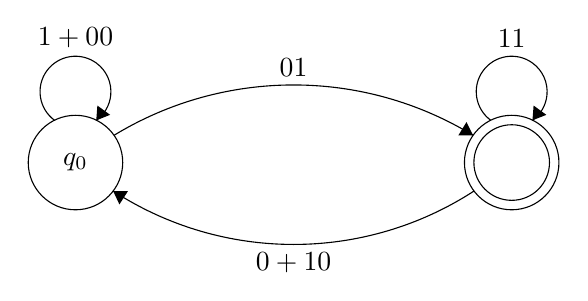
\begin{tikzpicture}[scale=0.2]
        \tikzstyle{every node}+=[inner sep=0pt]
        \draw [black] (17.9,-19.4) circle (3);
        \draw (17.9,-19.4) node {$q_0$};
        \draw [black] (45.6,-19.4) circle (3);
        \draw [black] (45.6,-19.4) circle (2.4);
        \draw [black] (43.209,-21.207) arc (-56.99933:-123.00067:21.039);
        \fill [black] (20.29,-21.21) -- (20.69,-22.06) -- (21.23,-21.22);
        \draw (31.75,-25.1) node [below] {$0+10$};
        \draw [black] (16.577,-16.72) arc (234:-54:2.25);
        \draw (17.9,-12.15) node [above] {$1+00$};
        \fill [black] (19.22,-16.72) -- (20.1,-16.37) -- (19.29,-15.78);
        \draw [black] (20.348,-17.67) arc (121.3332:58.6668:21.926);
        \fill [black] (43.15,-17.67) -- (42.73,-16.83) -- (42.21,-17.68);
        \draw (31.75,-13.97) node [above] {$01$};
        \draw [black] (44.277,-16.72) arc (234:-54:2.25);
        \draw (45.6,-12.15) node [above] {$11$};
        \fill [black] (46.92,-16.72) -- (47.8,-16.37) -- (46.99,-15.78);
    \end{tikzpicture}
\end{center}
Step 2: Remove accept state:
\begin{center}
    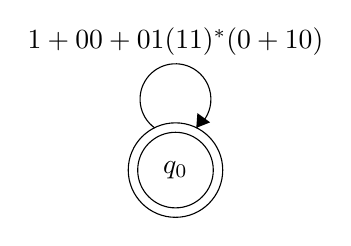
\begin{tikzpicture}[scale=0.2]
        \tikzstyle{every node}+=[inner sep=0pt]
        \draw [black] (37.6,-29.1) circle (3);
        \draw (37.6,-29.1) node {$q_0$};
        \draw [black] (37.6,-29.1) circle (2.4);
        \draw [black] (36.277,-26.42) arc (234:-54:2.25);
        \draw (37.6,-21.85) node [above] {$1+00+01(11)^*(0+10)$};
        \fill [black] (38.92,-26.42) -- (39.8,-26.07) -- (38.99,-25.48);
    \end{tikzpicture}
\end{center}
Therefore, the regular expression that represents this fsm is $(1+00+01(11)^*(0+10))^*$

\newpage
\section*{Problem 2}
\begin{proof}
    Assume $A$ is non-empty, and $N$ has $k$ states. Then the $k$ states in $N$ can be chained in a line to create a 
    unique word of length $k$ at most. Therefore, strings in A should have lengths at most $k$.\\*

    Now consider a DFA $D$ equivalent to $N$, we know that $D$ can have at most $2^k$ states using powerset construction.
    From $D$, we can construct another DFA $D_{reverse}$ that accepts $\overline{A}$ by reversing all accepting states to non-accepting states,
    and vice versa. Similar to $A$, because $D_{reverse}$ has at most $2^k$ states, $\overline{A}$
    can have strings with lengths of at most $2^k$\\*
\end{proof}

\section*{Problem 3}
\subsection*{(a)}
\begin{proof}
    Assume Palindromes over $\Sigma=\{a,b,c\}$ are regular languages, then there exists a DFA that accepts this language.\\*

    Consider an arbitrary palindrome over $\Sigma$, $p=a^mb^nc^{2k}b^na^m$, where $m,n,k \in \mathbb{N} $\\*

    Assume the DFA is in state $q_{mnk}$ when it reads $a^mb^nc^k$. Then from state $q_{mnk}$, the DFA must accept upon reading $c^kb^na^m$. Since DFA only has 
    a finite number of states, there must exists some state $q_{m'n'k'}$ for some $ m'\neq m, n' \neq n, k' \neq k, $ such that $q_{mnk}=q_{m'n'k'}$. This entails that from state $q_{m'n'k'}$, the machine
    will accept upon reading $c^kb^na^m$. However, $a^{m'}b^{n'}c^{k'}c^kb^na^m$ is not a palindrome, and we arrived at contradiction.\\*

    Therefore, by contradition, palindromes over $\Sigma=\{a,b,c\}$ are not regular language.
\end{proof}
\subsection*{(b)}
\begin{proof}
    Assume $\{10^110^210^3\dots0^{n-1}10^n1|n\ge 1\}$ is a regular language, then there exists a DFA that accepts it.\\*

    Consider an arbitrary string $10^110^210^3\dots10^k1, k \ge 1$. Assume the DFA is in state $q_k$ when it reads $10^110^2\dots0^{k-1}1$. Then from $q_k$, the machine will
    accept upon reading $0^k1$. Since DFA only has a finite number of states, then there must exists some $k' \neq k$ such that 
    $q_k = q_{k'}$. This entails that in state $q_{k'}$ the machine will accept upon reading $0^k1$. However, $10^110^2\dots0^{k'-1}10^k1$ is not in the language,
    and we have arrived at a contradiction.\\*

    Therefore, by contradiction, $\{10^110^210^3\dots0^{n-1}10^n1|n\ge 1\}$ is not a regular language.
\end{proof}
\end{document}